\documentclass[tikz,border=7pt]{standalone}
\usepackage{amsmath,amssymb}
\usetikzlibrary{arrows.meta,positioning,calc,fit,backgrounds}

% Muted academic palette shared with the nested-logit figure.
\definecolor{Ink}{HTML}{23384D}
\definecolor{Muted}{HTML}{607487}
\definecolor{Guide}{HTML}{D9E1E7}
\definecolor{DeepBlue}{HTML}{315F8C}
\definecolor{Teal}{HTML}{3E7773}
\definecolor{Amber}{HTML}{A66C32}
\definecolor{RailBlue}{HTML}{496A9B}
\definecolor{SoftGray}{HTML}{707982}

\tikzset{
	font=\sffamily,
	major/.style={-{Stealth[length=2.25mm,width=1.55mm]}, draw=Ink!88,
		line width=.95pt, rounded corners=1.4pt, line cap=round, line join=round},
	process/.style={-{Stealth[length=1.95mm,width=1.32mm]}, draw=Teal!88!Ink,
		line width=.76pt, rounded corners=1.3pt, line cap=round, line join=round},
	factor/.style={draw=Teal!60!Ink, line width=.58pt, line cap=round},
	relation/.style={draw=Ink!56, line width=.62pt, line cap=round},
	constraintlink/.style={-{Stealth[length=1.65mm,width=1.12mm]}, draw=SoftGray!72,
		line width=.58pt, dash pattern=on 2pt off 1.7pt, line cap=round},
	feedbackP/.style={-{Stealth[length=2.15mm,width=1.45mm]}, draw=RailBlue!88,
		line width=.82pt, rounded corners=2pt, line cap=round, line join=round},
	feedbackW/.style={-{Stealth[length=2.15mm,width=1.45mm]}, draw=Amber!90,
		line width=.82pt, rounded corners=2pt, line cap=round, line join=round},
	panel/.style={draw=Ink!34, fill=Ink!1.5, line width=.68pt,
		rounded corners=3pt, inner sep=6pt},
	panelhead/.style={text=white, rounded corners=1.6pt,
		minimum height=6.5mm, align=center, inner xsep=6pt,
		font=\bfseries\scriptsize},
	context/.style={draw=SoftGray!65, fill=SoftGray!5, line width=.68pt,
		rounded corners=2pt, minimum width=132mm, minimum height=8mm,
		align=center, inner sep=2.5pt, font=\scriptsize},
	objective/.style={line width=.82pt, rounded corners=2pt,
		minimum width=53mm, minimum height=14mm, align=center, inner sep=3pt},
	profitobjective/.style={objective, draw=RailBlue, fill=RailBlue!8},
	welfareobjective/.style={objective, draw=Amber, fill=Amber!8},
	switch/.style={circle, draw=Ink!62, fill=white, line width=.7pt,
		minimum size=7.5mm, inner sep=0pt, font=\bfseries\scriptsize, text=Ink},
	design/.style={draw=DeepBlue, fill=DeepBlue!8, line width=.92pt,
		rounded corners=2.2pt, minimum width=62mm, minimum height=13mm,
		align=center, inner sep=3pt},
	constraint/.style={draw=SoftGray!82, fill=SoftGray!5, line width=.68pt,
		rounded corners=1.8pt, minimum width=60mm, minimum height=18mm,
		align=center, inner sep=2.5pt, font=\scriptsize},
	ll/.style={draw=Teal, fill=Teal!7, line width=.76pt,
		rounded corners=2pt, minimum width=39mm, minimum height=15mm,
		align=center, inner sep=2.5pt, font=\scriptsize},
	qflow/.style={draw=Teal!88!Ink, fill=Teal!3, line width=.72pt,
		rounded corners=2pt, minimum width=128mm, minimum height=13mm,
		align=center, inner sep=3pt},
	metric/.style={line width=.72pt, rounded corners=1.8pt,
		minimum width=42mm, minimum height=15mm, align=center,
		inner sep=2.5pt, font=\scriptsize},
	financial/.style={metric, draw=RailBlue, fill=RailBlue!7},
	welfare/.style={metric, draw=Amber, fill=Amber!7},
	equity/.style={metric, draw=Teal, fill=Teal!7},
	optional/.style={draw=SoftGray!70, fill=white, line width=.58pt,
		dash pattern=on 2.2pt off 1.7pt, rounded corners=1.5pt,
		minimum width=58mm, minimum height=10mm, align=center,
		inner sep=2pt, font=\scriptsize},
	edgetag/.style={fill=white, fill opacity=.97, text opacity=1,
		rounded corners=.8pt, inner xsep=2.2pt, inner ysep=1.2pt,
		font=\scriptsize, text=Ink, align=center},
	note/.style={font=\scriptsize, text=Muted, align=center}
}

\begin{document}
	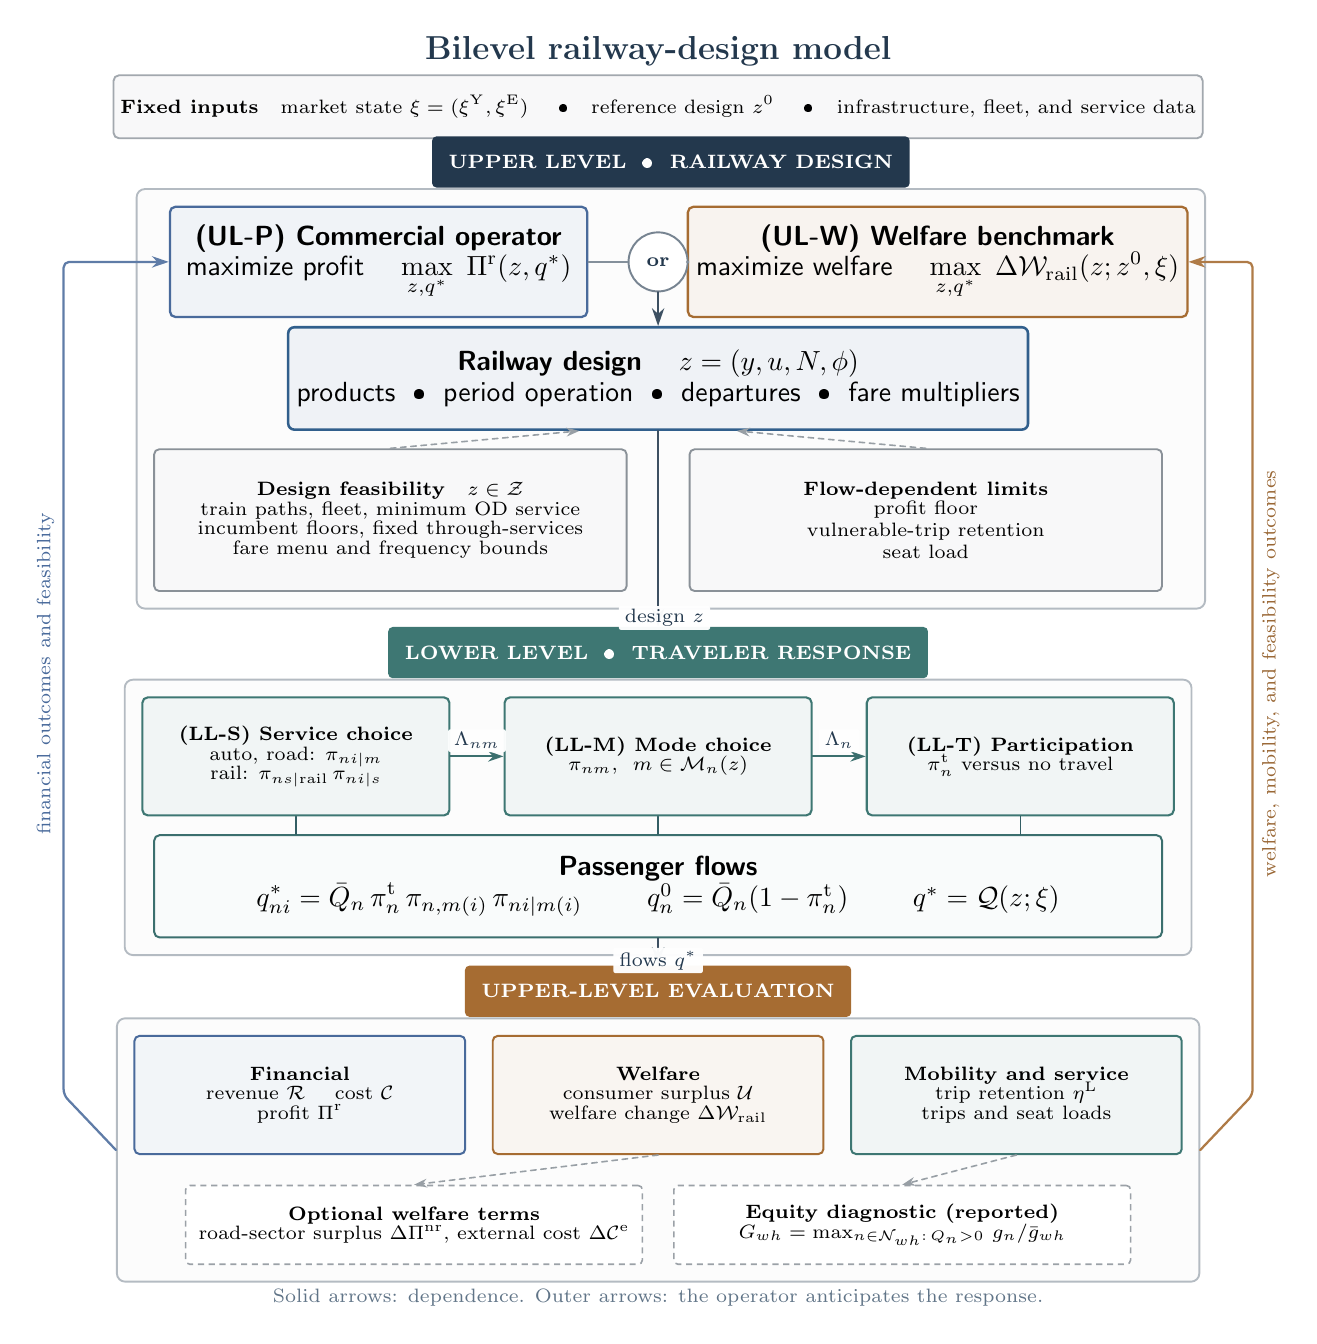
\begin{tikzpicture}[x=1cm,y=1cm]
		% Title and fixed inputs
		\node[font=\bfseries\large, text=Ink] at (0,1.95)
		{Bilevel railway-design model};
		\node[context] (inputs) at (0,1.25)
		{\textbf{Fixed inputs}\quad
			market state $\xi=(\xi^{\mathrm Y},\xi^{\mathrm E})$
			\quad\textbullet\quad reference design $z^0$
			\quad\textbullet\quad infrastructure, fleet, and service data};

		% Upper-level objective alternatives
		\node[profitobjective] (ulp) at (-3.55,-.72)
		{\textbf{(UL-P) Commercial operator}\\[-1pt]
			maximize profit \quad $\displaystyle\max_{z,q^*}\ \Pi^{\mathrm r}(z,q^*)$};
		\node[welfareobjective] (ulw) at (3.55,-.72)
		{\textbf{(UL-W) Welfare benchmark}\\[-1pt]
			maximize welfare \quad $\displaystyle\max_{z,q^*}\ \Delta\mathcal W_{\mathrm{rail}}(z;z^0,\xi)$};
		\node[switch] (orswitch) at (0,-.72) {or};
		\draw[relation] (ulp.east) -- (orswitch.west);
		\draw[relation] (orswitch.east) -- (ulw.west);

		\node[design] (design) at (0,-2.20)
		{\textbf{Railway design} \quad $z=(y,u,N,\phi)$\\[-1pt]
			products \;\textbullet\; period operation \;\textbullet\;
			departures \;\textbullet\; fare multipliers};
		\draw[major] (orswitch.south) -- (design.north);

		% Constraints that depend on z only (left) and on z and q* (right)
		\node[constraint] (feasible) at (-3.40,-4.00)
		{\textbf{Design feasibility}\quad $z\in\mathcal Z$\\[-1pt]
			train paths, fleet, minimum OD service\\[-1pt]
			incumbent floors, fixed through-services\\[-1pt]
			fare menu and frequency bounds};
		\node[constraint] (policy) at (3.40,-4.00)
		{\textbf{Flow-dependent limits}\\[-1pt]
			profit floor\\
			vulnerable-trip retention \\
			seat load };
		\draw[constraintlink] (feasible.north) -- ([xshift=-10mm]design.south);
		\draw[constraintlink] (policy.north) -- ([xshift=10mm]design.south);

		% Lower-level nested-logit response (inclusive values passed upward)
		\node[ll] (lls) at (-4.60,-7.00)
		{\textbf{(LL-S) Service choice}\\[-1pt]
			auto, road: $\pi_{ni\mid m}$\\[-1pt]
			rail: $\pi_{ns\mid\mathrm{rail}}\,\pi_{ni\mid s}$};
		\node[ll] (llm) at (0,-7.00)
		{\textbf{(LL-M) Mode choice}\\[-1pt]
			$\pi_{nm}$, \ $m\in\mathcal M_n(z)$};
		\node[ll] (llt) at (4.60,-7.00)
		{\textbf{(LL-T) Participation}\\[-1pt]
			$\pi^{\mathrm t}_n$ versus no travel};
		\draw[process] (lls.east) -- node[edgetag, above=1.2pt] {$\Lambda_{nm}$} (llm.west);
		\draw[process] (llm.east) -- node[edgetag, above=1.2pt] {$\Lambda_{n}$} (llt.west);

		\node[qflow] (qflow) at (0,-8.65)
		{\textbf{Passenger flows}\\[-1pt]
			$\displaystyle q^*_{ni}=\bar Q_n\,\pi^{\mathrm t}_n\,
			\pi_{n,m(i)}\,\pi_{ni\mid m(i)}$
			\qquad $q^0_n=\bar Q_n(1-\pi^{\mathrm t}_n)$
			\qquad $q^*=\mathcal Q(z;\xi)$};
		\draw[factor] (lls.south) -- (lls.south |- qflow.north);
		\draw[factor] (llm.south) -- (llm.south |- qflow.north);
		\draw[factor] (llt.south) -- (llt.south |- qflow.north);

		% Performance objects that depend on q*
		\node[financial] (financial) at (-4.55,-11.30)
		{\textbf{Financial}\\[-1pt]
			revenue $\mathcal R$ \quad cost $\mathcal C$\\[-1pt]
			profit $\Pi^{\mathrm r}$};
		\node[welfare] (welfare) at (0,-11.30)
		{\textbf{Welfare}\\[-1pt]
			consumer surplus $\mathcal U$\\[-1pt]
			welfare change $\Delta\mathcal W_{\mathrm{rail}}$};
		\node[equity] (equity) at (4.55,-11.30)
		{\textbf{Mobility and service}\\[-1pt]
			trip retention $\eta^{\mathrm L}$\\[-1pt]
			trips and seat loads};

		\node[optional] (optionalW) at (-3.10,-12.95)
		{\textbf{Optional welfare terms}\\[-1pt]
			road-sector surplus $\Delta\Pi^{\mathrm{nr}}$, external cost $\Delta\mathcal C^{\mathrm e}$};
		\node[optional] (diagnostic) at (3.10,-12.95)
		{\textbf{Equity diagnostic (reported)}\\[-1pt]
			$G_{wh}=\max_{n\in\mathcal N_{wh}:\,Q_n>0}\, g_n/\bar g_{wh}$};
		\draw[constraintlink] (welfare.south) -- (optionalW.north);
		\draw[constraintlink] (equity.south) -- (diagnostic.north);

		% Panel backgrounds are placed behind their contents.
		\begin{scope}[on background layer]
			\node[panel, fit=(ulp)(ulw)(design)(feasible)(policy)] (upperpanel) {};
			\node[panel, fit=(lls)(llm)(llt)(qflow)] (lowerpanel) {};
			\node[panel, fit=(financial)(welfare)(equity)(optionalW)(diagnostic)] (evalpanel) {};
		\end{scope}

		\node[panelhead, fill=Ink, anchor=south] (upperhead) at (upperpanel.north)
		{UPPER LEVEL \;\textbullet\; RAILWAY DESIGN};
		\node[panelhead, fill=Teal, anchor=south] (lowerhead) at (lowerpanel.north)
		{LOWER LEVEL \;\textbullet\; TRAVELER RESPONSE};
		\node[panelhead, fill=Amber, anchor=south] (evalhead) at (evalpanel.north)
		{UPPER-LEVEL EVALUATION};

		% Cross-level dependence: central downward path and mirrored return paths.
		\draw[major] (design.south) -- (lowerhead.north);
		\node[edgetag] at ($(upperpanel.south)!.5!(lowerhead.north)$)
		{design $z$};
		\draw[major] (qflow.south) -- (evalhead.north);
		\node[edgetag] at ($(lowerpanel.south)!.5!(evalhead.north)$) {flows $q^*$};

		\draw[feedbackP] (evalpanel.west) -- (-7.55,-11.30) -- (-7.55,-.72) -- (ulp.west);
		\draw[feedbackW] (evalpanel.east) -- (7.55,-11.30) -- (7.55,-.72) -- (ulw.east);
		\node[note, rotate=90, text=RailBlue] at (-7.78,-5.95)
		{financial outcomes and feasibility};
		\node[note, rotate=90, text=Amber!90!Ink] at (7.78,-5.95)
		{welfare, mobility, and feasibility outcomes};

		\node[note] at (0,-13.88)
		{Solid arrows: dependence. Outer arrows: the operator anticipates the response.};
	\end{tikzpicture}
\end{document}
